\subsection{Word vs. Instance-Based Induction}
\label{sec:typevsinstance}

\begin{figure}[h] \centering
  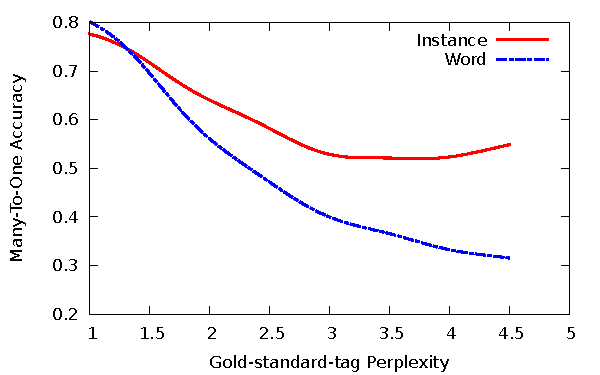
\includegraphics[width=\columnwidth]{ksmooth-f.pdf} 
  \caption{Regression lines for the word and instance based models on the \mto\
    accuracy vs {\em GP} plot for the PTB.} 
  \label{fig:perplexity}
\end{figure}

In this section we compare the output of a word-based and an
instance-based POS induction system.  We use the state of the art
word-based induction system described in
\cite{yatbaz-sert-yuret:2012:EMNLP-CoNLL} which achieves
\ftmto\ \mto\ and \ftvm\ \vm\ on the PTB.

We propose the gold-tag perplexity of a word as a measure of its
degree of ambiguity defined as follows:
\begin{equation*} \label{eq:tag-perp}
GP(w) = 2^{H(p_w)} = 2^{-\sum_{t} p_w(t)log_2 p_w(t)}
\end{equation*}
\noindent where $w$ is a word, $t$ is a tag, $p_w$ is the gold POS tag
distribution of the word $w$ and $H(p_w)$ is the entropy of the $p_w$
distribution.  A $GP$ of 1 for a word $w$ indicates that $w$ is always
associated with the same POS tag.  A word with $N$ equally probable
tags would have a $GP$ of $N$.

Figure~\ref{fig:perplexity} plots the gold-tag perplexity versus the
smoothed \mto\ accuracy for the word-based and the instance-based POS
induction system.  To compose the plot, we find the best mapping from
the induced clusters to the gold-standard tags, then we compute the
\mto\ accuracy for each word using this mapping and plot the \mto\ as
a function of the word's $GP$.  We use the Nadaraya-Watson kernel
regression estimate \cite{nadaraya1964estimating,watson1964smooth}
with normal kernel of bandwidth 1.0 to obtain smooth regression lines.

Figure~\ref{fig:perplexity} shows that the performance of the
instance-based induction model does not degrade as much as the
word-based model as the ambiguity of the words increase.  However,
only 14.94\% of the instances in the PTB consists of words with GP
greater than 1.5 and 45.71\% consists of words with GP exactly 1.
Thus, the overall accuracy numbers do not adequately reflect the
improvement on highly ambiguous words.

%% In the next section we apply the instance based model on 19 corpora in 15
%% different languages. 

%% Due to the one-tag-per-word nature of POS induction, the
%% type based model significantly outperforms the instance based one on the
%% unambiguous words.  Instance based model performs significantly better than the
%% type based model on the ambiguous words and assigns 1.34 tags per word.  
%% \subsection{Clustering Concatenation of Word and Context Embeddings (${\bf W}\oplus{\bf S}$)}
%% \label{sec:clustering-c}
%% Two models presented in earlier sections perform POS induction either
%% by assuming (Section~\ref{sec:clustering-w}) or discarding
%% (Section~\ref{sec:clustering-c}) the one-tag-per-word assumption.  In
%% this section we define a sparse-instance based model which clusters the
%% concatenation of ${\bf W}$ and ${\bf S}$ embeddings.  This model not
%% only tends to put instances of a word into the same cluster but
%% also performs instance based clustering by incorporating the word
%% and context information together.
%%
%% Similar to the previous models, we generate ${\bf W}$ -- ${\bf S}$
%% pairs as the input to S-CODE.  For each observed ${\bf W}$ -- ${\bf
%%   S}$ pair in the S-CODE input, corresponding 25-dimensional $\phi_w$
%% and $\psi_c$ embeddings are concatenated to create a 50-dimensional
%% representation.  We used the same experimental setting of the previous
%% section and predict the instance clusters according to the majority
%% cluster-id of the corresponding pairs.  The many-to-one accuracy of
%% this model is \wsxymto\ and the V-measure is \wsxyvm\ .
%% 
%% Table~\ref{tab:bins} presents the performance of the ${\bf
%%   W}\oplus{\bf S}$ based model over the subsets and it achieves
%% statistically better \mto\ than both of the ${\bf W}$ and ${\bf S}$
%% based models on ambiguous words.  Due to the bias towards to the
%% sparse clustering, sparse-instance based model statistically improves the
%% \mto\ accuracy on unambiguous words compared to the ${\bf S}$ based
%% model but it still can not achieve the performance of the ${\bf W}$
%% based model.  The ${\bf W}\oplus{\bf S}$ based model constructs instance 
%% based clusters that tend to assign instances of a word into the
%% same cluster which leads to a smaller average $GP$ than the ${\bf S}$
%% based model as shown in Table~\ref{tab:bins}.
%%
%% We don't really need this part
%% \subsubsection{Paradigmatic vs Syntagmatic Representations of Word Context}
%% \label{sec:bigram-instance}
%% In order to compare the instance clustering performance of the
%% paradigmatic and the syntagmatic context representations we use the
%% same 4 models defined in Section~\ref{sec:bigram-type}.  Following the
%% previous section we concatenate the 25-dimensional $\phi_x$ and
%% $\psi_y$ ($\psi_{y_{1}}$ and $\psi_{y_{2}}$ in the fourth model)
%% embeddings of the corresponding observed pairs (tuples in the fourth
%% model) and represent the first three models outputs with a
%% 50-dimensional vectors (75-dimensional vectors in the fourth model).
%% The resulting vectors are clustered using k-means algorithm with 128
%% restarts.
%% \begin{table}[ht]
%% \centering
%% \small
%% \caption{Accuracies of the instance based S-CODE models on the gold-tag
%%   perplexity separated subsets.}
%% \begin{tabular}{|l|l|l|l|}
%% \hline
%% Model & \specialcell{$GP < 1.75$\\$89\%$} & \specialcell{$GP \ge 1.75$\\$11\%$} & \specialcell{$GP \ge 1.0$\\$100\%$}\\
%% \hline
%% $X$ (word) - $Y$ (left bigram) & .5950 (.0051) & .4783 (.0005) & .5821 (.0041)\\
%% $X$ (word) - $Y$ (right bigram) & .6239 (.0049) & .3075 (.0153) & .5891 (.0046)\\
%% $X$ (word) - $Y$ (left and right bigram concatenation) & .7523 (.0065) & .4492 (.0240) & .7190 (.0049)\\
%% $X$ (word) - $Y_1$, $Y_2$ (left and right bigrams) & .6697 (.0065) & .4579 (.0052) & .6464 (.0051)\\
%% $X$ (word) - $Y$ (random substitutes) & .7322 (.0079) & .4671 (.0174) & .7030 (.0073)\\
%% \hline
%% \end{tabular}
%% \label{tab:instances}
%% \end{table}
